% Exam package: Instructions & student name

\documentclass{exam}
\usepackage{graphicx}

\pagestyle{headandfoot}
\runningheader{Introduction to Information Technology}{}{Midterm}
\runningheadrule
\runningfooter{}{Page \thepage\ of \numpages}{}

% To hide points
% \nopointsinmargin
% \pointformat{}

\begin{document}
\addpoints

\begin{center}
    \vspace{2in}
    {\Large Introduction to Information Technology Midterm}
    \vspace{1.8in}

    \begin{figure}[h]
        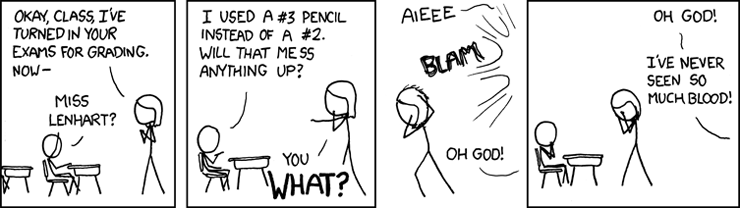
\includegraphics[width=\linewidth]{scantron.png}
    \end{figure}

    \vspace{1.3in}
    \fbox{\fbox{\parbox{5.5in}{\centering
            \textbf{Read carefully before starting the test:}
            \begin{itemize}
                \item Answer the questions using pencil or
                    a blue or black pen.
                \item You can use a calculator if you want, but it can't have internet access.
                \item Answer the questions in the spaces provided on the
                question sheets. If you run out of room for an answer,
                continue on the back of the page
                \item You are allowed one sheet 11.5 x 8in paper (or smaller) of handwritten notes
            \end{itemize}}}}

\vspace{0.2in}
\end{center}

\makebox[\textwidth]{\textsc{Full name:}\enspace\hrulefill}

\vspace{0.2in}

\makebox[\textwidth]{\textsc{Computing ID:}\enspace\hrulefill}

\vspace{0.2in}
\gradetable[h][pages]
\newpage

\begin{questions}
\section{True or False (10 Points)}
\question[1] T / F : An analog signal has limited precision.
\question[1] T / F : The primary key is a field in a database table.
\question[1] T / F : Network packets can be sent independently of each other in parallel.
\question[1] T / F : A Wi-Fi network is an example of a PAN.
\question[1] T / F : Programming Languages can express things binary can't.
\question[1] T / F : Boolean Logic is the basis of computer circuit design.
\question[1] T / F : Artificial Neural Networks are trained by adjusting the weights of the network.
\question[1] T / F : RAM is a form of computer storage.
\question[1] T / F : The primary use of CSS is to define the content on a webpage.
\question[1] T / F : Infrastructure as a Service is the most general cloud service.

\section{Multiple Choice (10 Points)}
\question[1] Which of the following best describes the Internet?
\begin{choices}
    \choice A global network of interconnected computers and servers.
    \choice A single, centralized server storing all online information.
    \choice A private network used by government agencies only.
    \choice A collection of offline computer databases.
\end{choices}
\question[1] Which technology allowed computers to shrink drastically in size:
\begin{choices}
    \choice The Motherboard
    \choice The Vacuum Tube
    \choice The Transistor
    \choice None of the above
\end{choices}
\question[1] Which component has the primary job of performing computations:
\begin{choices}
    \choice The GPU
    \choice The CPU
    \choice Both A and B
    \choice Neither A nor B
\end{choices}
\question[1] Which of the following is not a standard boolean operator:
\begin{choices}
    \choice $\land$
    \choice $\Xi$
    \choice $\lor$
    \choice $\lnot$ 
\end{choices}

\newpage
\question[1] Which layer of the internet protocol suite determines where information is sent:
\begin{choices}
    \choice The Application Layer
    \choice The Transport Layer
    \choice The Internet Layer
    \choice The Link Layer
\end{choices}

\question[1] Which is not a core language of the web:
\begin{choices}
    \choice Fortran
    \choice JavaScript
    \choice HTML
    \choice CSS
\end{choices}
\question[1] What is the purpose of Diffe-Hellman Key Exchange:
\begin{choices}
    \choice It translates boolean logic to electronic signals.
    \choice It allows you to establish a new secure connection on the internet.
    \choice It creates secure passwords.
    \choice It produces webpages from HTML. 
\end{choices}
\question[1] Which component of the Model-View-Controller Pattern is generally controlled solely by the frontend:
\begin{choices}
    \choice The Controller
    \choice The Model
    \choice The View
    \choice All of the above
\end{choices}
\question[1] Which is a class of learning in machine learning:
\begin{choices}
    \choice Reinforcement learning
    \choice Rule learning
    \choice Support Vector Machines
    \choice Active learning
\end{choices}
\question[1] Database management systems include:
\begin{choices}
    \choice A way to store data
    \choice A way to access data
    \choice A way to update data
    \choice All of the above
\end{choices}

\bonusquestion[1] In lecture, I have often mentioned where I am from. Which city is it (roughly):
\begin{choices}
    \choice Cincinnati
    \choice Portland
    \choice Chicago
    \choice Boston
\end{choices}

\newpage
\section{Show Your Work (21 Points)}
\question[3] Convert 117 to binary:
\vspace{4.5in}
\question[3] Convert 1001001 to decimal:
\newpage 

\question[5] Produce the truth table for the following logical expression:
\[
((X \iff Z) \land Y) \lor Z
\]
\vspace{4in}

\question[5] Is $\lnot (P \lor Q)$ logically equivalent to $(\lnot P) \lor (\lnot Q)$? Show why or why not and explain:

\newpage
\question[5] The following network has been trained to predict how many peppers will grow on a plant by September based on the hardiness zone and month it was planted in. I'm going to plant my peppers in Charlottesville (zone 7) in May (month 5). Using this network, calculate the value of each neuron based on how I'm planting my pepper plant and tell me how many peppers I should expect based on the network's output.

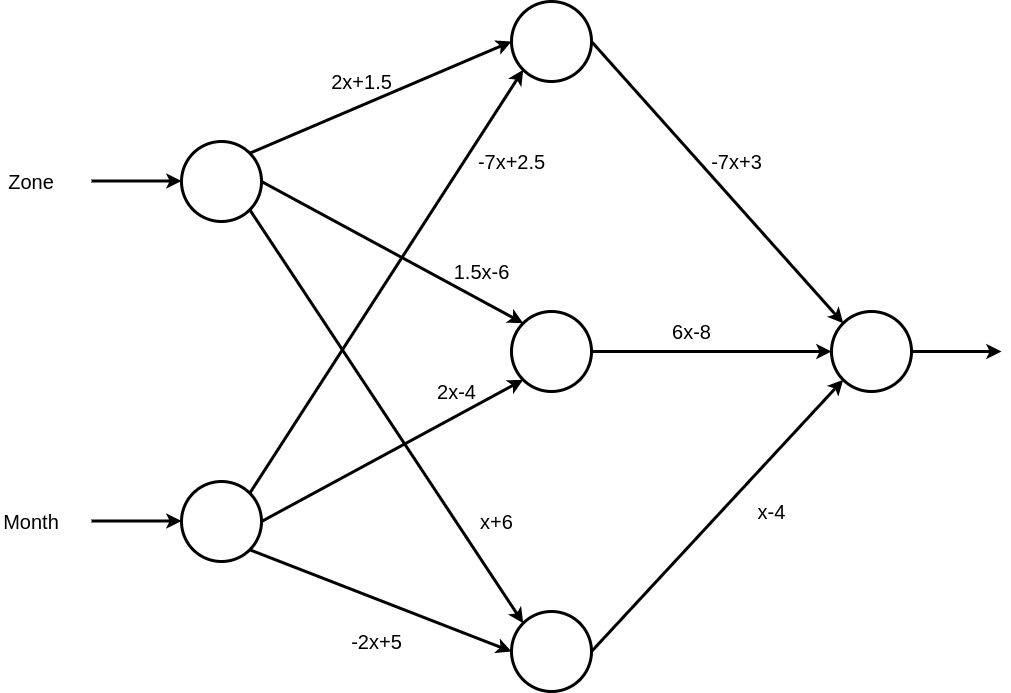
\includegraphics[width=\linewidth]{network.png}

\newpage

\section{Short Answer (19 Points)}
\question In lecture, I described the CPU as ``the brain of the computer''. 
\begin{parts}
\part[3] Describe the ways in which the CPU fits this description:
\vspace{1.5 in}
\part[2] Other parts of the computer are responsible for activities we would relate to the brain, name one component that would fit this description and describe why:
    
\end{parts}

\vspace{2in}

\question[3] Describe two benefits of cloud computing:
\newpage

\question[2] Describe two ways in which primary keys are important
\vspace{2in}

\question[3] When we say a model ``learns'' in machine learning, what do we mean?
\vspace{2in}


\bonusquestion[2] One of the multiple choice questions was generated by a transformer model. Pick which question you think it was and explain. (1 point for choosing the right question and 1 point for your explanation. You don't have to choose the right one to get the second point. Just explain your reasoning based on our discussions of machine learning.)
\end{questions}

\end{document}